% https://tex.stackexchange.com/a/354033
\documentclass[11pt]{beamer}
\usepackage[english]{babel}
\usepackage{fontenc}
\usepackage[latin1]{inputenc}
\mode<presentation>
{
\usetheme{Berkeley}
\setbeamercovered{transparent}
}

%Title
\title[Example]{Example}
\usepackage{tikz}

%*DOCUMENT*
\begin{document}

%*INTRODUCTION*
\section{Introduction}

%Trees
\subsection[Trees]{Trees}
\begin{frame}
\frametitle{Introduction:\\ Trees}
\begin{columns}[t]
 \begin{column}{0.48\textwidth}
 \uncover<1,2>{
  \begin{block}{Tree1}
   \begin{figure}
    \centering
        \includegraphics[width=\linewidth]{example-image-duck}
        \label{fig:a}
   \end{figure}
  \end{block}}      
 \end{column}
 \begin{column}{0.48\textwidth}
 \uncover<1>{
  \begin{block}{Tree2}
  \begin{figure}
    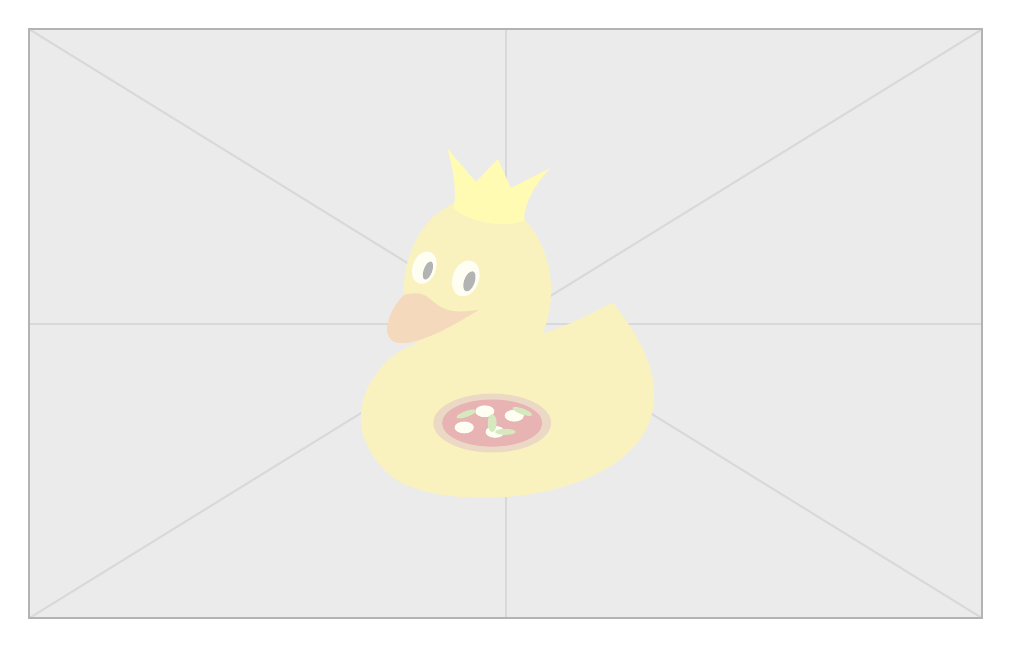
\begin{tikzpicture}
    \node[anchor=south west,inner sep=0] (B) at (4,0) {\includegraphics[width=\linewidth]{example-image-duck}};
    \only<2>{%
        \fill [draw=none, fill=white, fill opacity=0.7] (B.north west) -- (B.north east) -- (B.south east) -- (B.south west) -- (B.north west) -- cycle;
    }
    \end{tikzpicture}
    \end{figure}
  \end{block}}
 \end{column}
\end{columns}
\end{frame} 

\end{document}
